

\chapter{Lösungsdesign}

Das Lösungsdesign beinhaltet die Grundlagen für die erfolgreiche Umsetzung des Prototyps. Darin wird basierend auf den Anforderungen und der Aufgabenstellung die Software-Architektur definiert. Wäh\-rend dies auf einer hohen Abstraktionsebene geschieht, erfolgt in einem nächsten Schritt der Entwurf und das Design der Software. Dabei dient die Architektur als Leitplanke, welche zusammen mit der Recherche über den aktuellen Stand der Technik (\autoref{literatur}) zu einem konkreten Entwurf führt.

% ----------------------------------------------------------------

\section{Architektur}\label{architecture}

% ----------------------------------------------------------------

Der Architektur-Entwurf betrachtet die zu entwickelnde Software aus einer abstrakten Sicht. Das Ziel ist eine grundsätzliche Übersicht über die Software, deren Komponenten, Schnittstellen und auch deren Verteilung.


Basierend auf den Anforderungen (\autoref{sec:anforderungen}) an den zu entwickelnden Prototypen, wird im folgenden Abschnitt die zugrundeliegende Architektur-Entwurf ausgeführt. Die Ar\-chi\-tek\-tur-\-Ent\-schei\-dung\-en bilden die Grundlage für die Designentscheidungen für den Soft\-wa\-re-\-Ent\-wurf. Grundlegend orientieren wir uns bei dem Entwurf an dem \textit{4+1 Schichtenmodell}. \\\cite{kruchten1995architectural}.


%\url{https://www4.in.tum.de/misc/perlen/perlen-folien/PDW_Architektur_IK_Druckversion.pdf}\\
%\url{http://www.edv-buchversand.de/chapter.php?cnt=getchapter&id=ha-41215_2.pdf}\\


\subsection{Kontextsicht}
    \begin{figure}[ht]
    \centering
    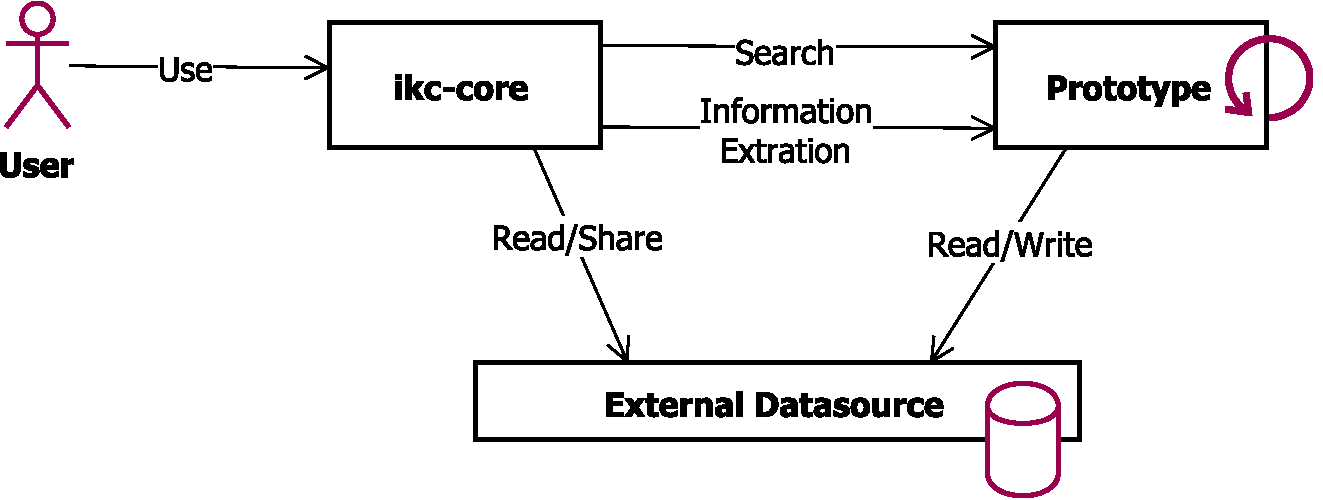
\includegraphics[width=1\textwidth]{BDA_Context}
    \caption{Kontextsicht}
    \label{fig:kontextsicht}
    \end{figure}
 
 Die \autoref{fig:kontextsicht} gibt einen Überblick über den Kontext des zu entwickelnden Prototypen:
 Der \texttt{ikc-core} nutzt den Prototypen zur Erweiterung seiner Funktionalität. Damit können die Hauptanforderungen, die Volltextsuche und die Extraktion von Schlüsselwörter, abgedeckt werden. Diese beiden Funktionen sind für den Benutzer über das \texttt{UserInterface} innerhalb des \gls{ikc-core} verfügbar. Sowohl der \gls{ikc-core} als auch der Prototyp haben Zugriff auf die externen Datenquelle. Der Prototyp hat dort die Quellen für die Dateiinhalte und hält dort auch Indizes für die Volltextsuche und die Schlü\-ssel\-wort-Ex\-trak\-tion.
 



\subsection{Einflussfaktoren}\label{einflussfaktoren}

Basierend auf dem Kontext des \gls{ikc-core}, dem Scope und der funktionalen und nichtfunktionalen Anforderungen beeinflussen verschiedenen Faktoren den Architektur Entwurf.

\begin{longtable}{|p{4cm}|p{8.5cm}|}

  \hline
    Faktor &  Beschreibung \\\hline
    Browseranwendung & Der \gls{ikc-core} ist als clientseitige Browseranwendung aufgebaut und kann bis anhin grundsätzlich ohne serverseitige Logik genutzt werden. %Funktionale Erweiterungen mit Hilfe von zusätzlicher zentralen Services sind in Entwicklung. Diese betreffen jedoch keine grundlegenden Funktionen der Applikation.
    \\\hline
    Mehrplatz-Nutzung & Soll der \gls{ikc-core} in einer Mehrplatz-Umgebung genutzt werden, ist eine Synchronisation auf \gls{Dropbox} notwendig. Diese muss vom Benutzer explizit angegeben und authorisiert werden.\\\hline
    Hardware Infrastruktur & Die Server-Infrastruktur des Departements Informatik (\textit{enterpriselab}) bietet die Ressourcen, auf welchen die Webanwendung läuft. Dazu werden zwei virtuelle \gls{Ubuntu}-Server verwendet. Die Entwicklung und die Produktion sind somit komplett voneinander getrennt.\\\hline
    
    Software Infrastruktur & Als Basis für Applikationsverteilung auf die Entwicklungs- und Produktions-System wird \gls{Dokku} in Kombination mit \gls{Gitlab CI} verwendet. Änderungen so direkt aus dem Versionskontrollsystem verteilt. Die Software wird als \gls{Docker}-Container ausgeliefert und anschliessend als dedizierte Applikation innerhalb des \gls{Dokku}-Frameworks gestartet.\\\hline
    
    Programmiersprachen & Als Programmiersprache wird \gls{Typescript} verwendet. Anders als andere Webprogrammiersprachen wie \gls{Javascript} ermöglicht sie die Verwendung von Sprachkonstrukten der Typisierung, wie zum Beispiel Klassen oder Vererbung. Durch den Typescript-Kompiler wird der Code für die Ausführung in reinen \gls{Javascript} Code übersetzt. Mit der Verwendung der \gls{Node}-Plattform kann \gls{Typescript} auch für eine Server Anwendung verwendet werden. Dadurch steigt sowohl die Wiederverwendbarkeit als Skalierbarkeit.\\\hline
    
    Kommunikation & Für eine allfällige Kommunikation zwischen dem \gls{ikc-core} und einer serverseitigen Erweiterung wird über einen Websocket abgehandelt. Dadurch wird eine beidseitige Kommunikation ermöglicht. \\\hline
    
    UI-Framework & Die Verwendung des \gls{React}-Frameworks ermöglicht den modularen Aufbau des \texttt{ikc-core}. Die gesamte Oberfläche ist in verschiedene Elemente aufgeteilt, welche über den Applikationzustand gesteuert werden. Eingaben des Benutzers werden durch die verschiedenen \texttt{UI Services} abgearbeitet und resultieren in einem aktualisierten Applikationszustand. Der unidirektionale Datenfluss sorgt für die klare Trennung der Verantwortlichkeiten innerhalb der \texttt{UI Services}. \\\hline
    
    Datenhaltung & Der \gls{ikc-core} nutzt keine zentralen Services für die Persistenz von den Daten der Benutzer oder deren Applikations-Konfiguration. Es werden die lokalen Ressourcen oder externe Datenquellen wie \gls{Dropbox} verwendet. \\\hline
    \caption{Einflussfaktoren}
  \label{tab:einflussfaktoren}
\end{longtable}


%Der \gls{ikc-core} ist primär eine Browserapplikation, der Grossteil der verwendeten Komponenten läuft ebenfalls clientseitig. Die Kommunikation mit serverseitigen Services funktioniert über REST-Schnittstellen oder WebSockets. Darunter gehört beispielsweise eine Schnittstelle mit \gls{Evernote}. Dies hat insbesondere den Grund, dass durch die Nutzung des \gls{ikc-core} keine zusätzliche Persistenz eingeführt wird. Darum sind keine zentralen Applikations- und Datenserver notwendig.

%Dies schränkt die Architektur insoweit ein, dass Komponenten mit kritischer Funktionalität oder Leistung möglichst gekapselt und entkoppelt sind. Nur in diesem Fall ist gewährleistet, dass eine entsprechende Komponente, falls notwendig, auch auf einer Server-\-Um\-geb\-ung laufen kann.

\subsection{Architekturtreiber}
Zwei elementare Architekturtreiber beeinflussen die Konzeption des Prototyps. Diese wurden bereits weiter oben als Einflussfaktor (\autoref{einflussfaktoren}) erwähnt, haben jedoch auch für den Prototyp eine zentrale Bedeutung.

\begin{itemize}
    \item \textbf{Entkopplung und Wiederverwendbarkeit}:
    Module und Komponenten sind entkoppelt voneinander. Dadurch können diese innerhalb der Applikation, oder auch für zukünftige Projekte, leicht wiederverwendet werden. Bei Performance-Engpässen ist es weiter möglich, bestimmte Module auszulagern, dies sowohl lokal innerhalb der Client-Applikation, als auch extern auf eine Server-Umgebung.
    \item \textbf{Verhinderung von zusätzlicher Persistenz}:
    Applikationsdaten- und Konfiguration sind stets lediglich von den bestehenden Datenquellen zu beziehen. Hierbei handelt es sich entweder um den lokalen Cache des Benutzers oder die entsprechende externe Datenquelle. Durch diesen Umstand kann viel Zeit für die Entwicklung und die Absicherung einer Persistenz-Infrastruktur gespart werden. Der Benutzer hat so zusätzlich immer eine transparente Kontrolle über den Speicherort und auch den Inhalt der eigenen Daten.
    \item \textbf{Inspiration durch React und Flux}: Wie in \autoref{react} bereits erwähnt, arbeitet React im Hintergrund mit einer eigenen Implementation von Flux. Dieser orientiert sich stark am funktionalen Programmier-Paradigma: Innere Zustände, also Variabeln, sind wann immer möglich zu verhindern. Dies wirkt allfälligen Seiteneffekten entgegen, macht den Code so nachvollziehbarer. Auch der unidirektionale Datenfluss strebt ähn\-liche Ziele an. Diese Überlegungen begleiteten die Entwicklung ständig. So sind an vielen Orten Programmierkonstrukte zu finden, welche prinzipiell verwandte Ansätze verfolgen.
\end{itemize}

\subsection{Architekturziele}

Der zu entwickelnde Prototyp baut auf dem bestehenden \gls{ikc-core} auf. Dabei soll das Augenmerk weiterhin auf den bereits bestehenden Eigenschaften der Architektur, insbesondere der Modularität und der Erweiterbarkeit, gehalten werden. Dies ist im Kontext des zugrundeliegenden Forschungsprojekts von hoher Wichtigkeit. Die Vergangenheit hat gezeigt, dass eine solide aber gleichzeitig auch anpassungsfähige Basis ein kritischer Faktor für die agile Weiterentwicklung ist. Einzig unter diesen Voraussetzungen ist es möglich auf die stetig ändernden Anforderungen entsprechend zu reagieren.

Die wichtigsten Ziele der Architektur sind in folgender Tabelle (\autoref{tab:architekturziele}) kurz erläutert:

\begin{longtable}{|p{4.5cm}|p{8.5cm}|}

  \hline
    Ziel &  Beschreibung \\\hline
    Modularität & Die verschiedenen Komponenten sind auswechselbar und an anderen Orten wiederverwendbar. Eine lose Kopplung und eine hohe Kohäsion innerhalb der Komponenten und deren Klassen ist dafür vorausgesetzt.\\\hline
    Erweiterbarkeit & Die Komponenten sind offen für Erweiterungen. Ein Ausbau der Funktionalität ist stets möglich.\\\hline
    Skalierbarkeit & Durch Bildung von Schichten ist es möglich einzelne Komponenten horizontal zu skalieren. Das bedeutet, dass mehrere gleiche Services beispielsweise sich einzelne Aufgaben teilen können. Dafür sind diverse Szenarien denkbar. Die Performance kann so an bestimmten Stellen optimiert werden.\\\hline
%    Vorbereitung Multiuser-Betrieb & \\\hline
    Benutzerfreundlichkeit & Bezüglich der Benutzeroberfläche ist es wichtig, dass der Benutzer immer über die Abläufe im Hintergrund informiert wird. Insbesondere bei der aufwändigen Verarbeitung von grossen Datenmengen, ist er Benutzer nie gehindert oder gar blockiert seine Arbeit mit dem Prototypen fortzusetzen. Sind die Resultate verfügbar, wird er benachrichtigt und kann auf deren Basis weiterarbeiten.\\\hline
    Performance & \\\hline
    \caption{Ziele der Architektur}
  \label{tab:architekturziele}
\end{longtable}

% Performance, Stresstest, Flexibilität, Erweiterbarkeit, Benutzerfreundlichkeit
% anderer Kontext, ...
%Entkoppelt, einfach erweiterbar, modularisiert, microservices, skalierbar


\subsection{Bausteinsicht}
Die \autoref{fig:bausteinsicht} beschreibt die Bausteinsicht der Architektur des Prototypen. Darin werden die verschiedenen Komponenten und Module und deren Beziehungen untereinander aufgezeigt. Hierbei werden drei verschiedene Abstraktionslevel unterschieden. 

\begin{figure}[H]
\centering
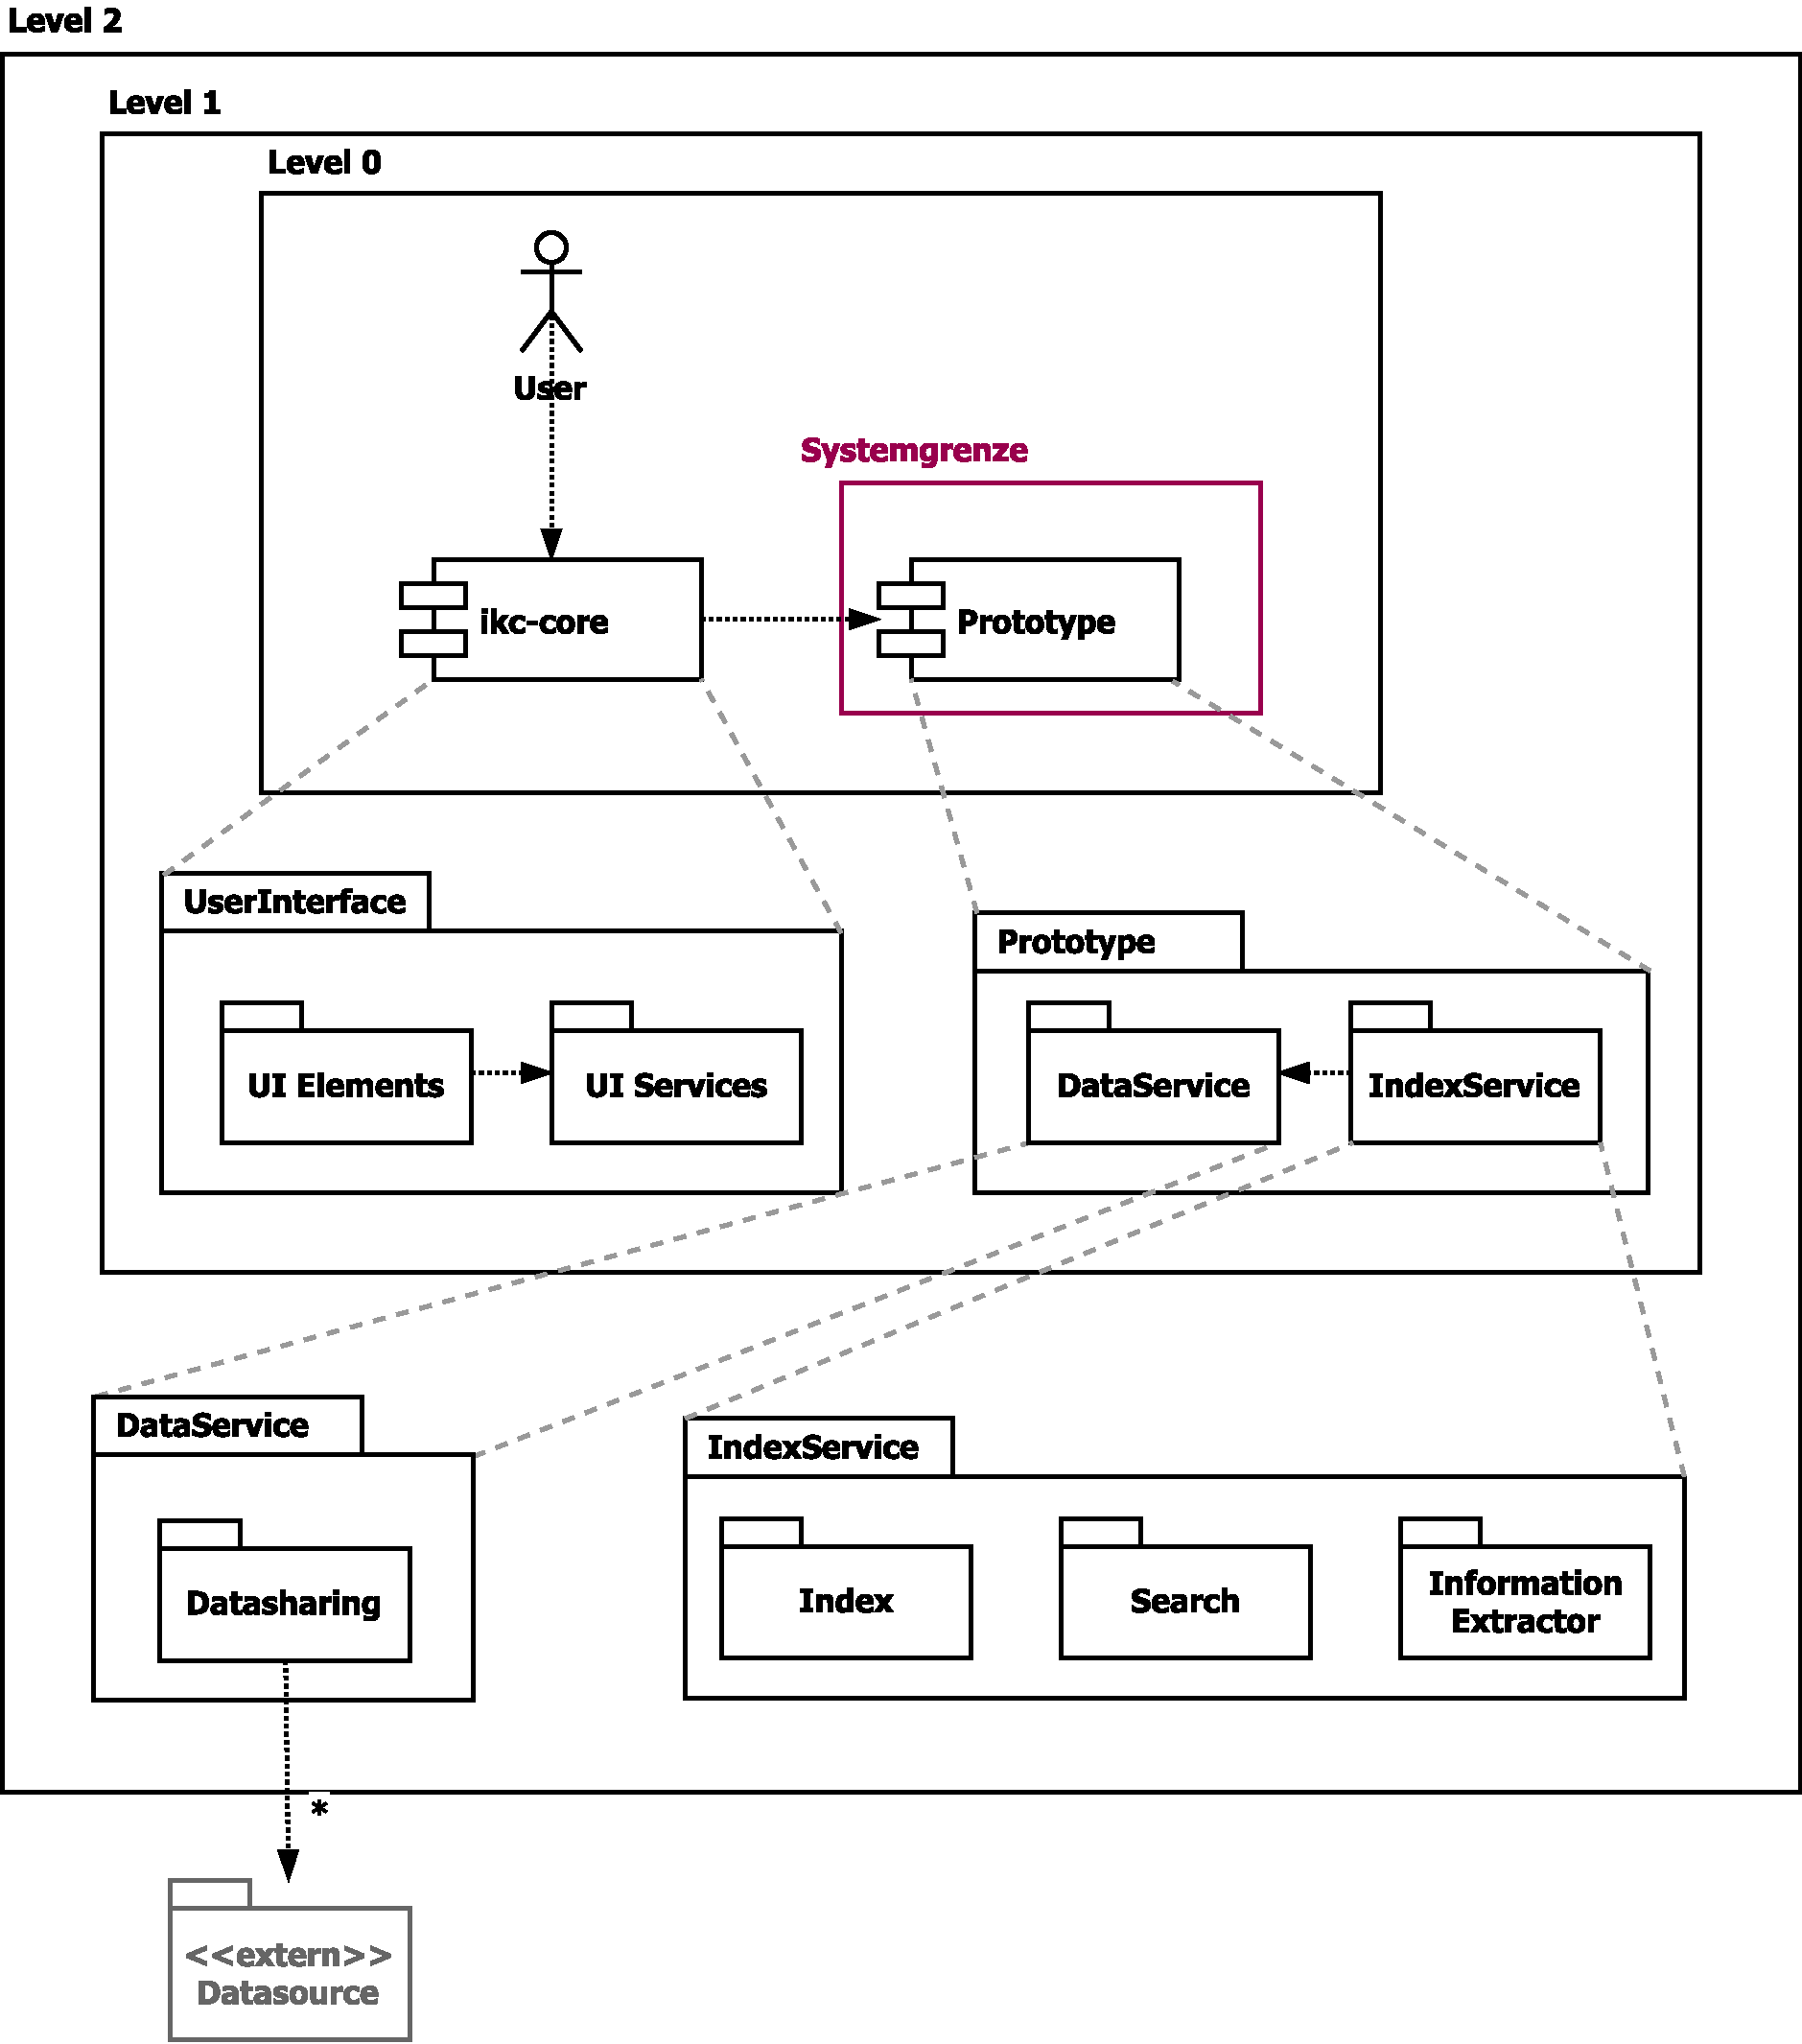
\includegraphics[width=1\textwidth]{BDA_Whitebox}
\caption{Bausteinsicht}
\label{fig:bausteinsicht}
\end{figure}

Nachfolgend werden diese näher erläutert.

\subsubsection{Bausteinsicht Level 0}
Innerhalb des \texttt{Level 0} werden die Zusammenhänge zwischen dem \texttt{User}, dem \texttt{ikc-core} und dem \texttt{Prototypen} aufgezeigt. Ebenfalls ist die Systemgrenze zwischen der bestehenden und der zu erstellenden Komponente ersichtlich. Die Systemgrenze grenzt den Kern des Prototyps ein.

\sssubsection{User}
Wie bisher hat der Benutzer über die Benutzeroberfläche des \gls{ikc-core} Zugriff auf alle Funktionalitäten. Die Zusatzfunktionen, welche durch den Prototyp zur Verfügung gestellt werden, sind für den Benutzer in der Suchfunktion und den extrahierten Schlüsselwörter ersichtlich.

\sssubsection{ikc-core}
Neben den bisherigen Funktionalitäten nutzt der \texttt{ikc-core} zusätzlich die neuen Funktionen, welche vom Prototypen zu Verfügung gestellt werden. Dazu zählt die Volltextsuche und die Schlüs\-sel\-wort-\-Ex\-trak\-tion. Er besteht prinzipiell aus verschiedenen \texttt{UI\-Ele\-ments} welche \texttt{UI\-Ser\-vices} nutzen um zugrundeliegende Logik zu kapseln. In dieser Logik soll der \texttt{Prototype} integriert werden.

\sssubsection{Prototype}
Die Komponente \texttt{Prototype} kapselt die essentiellen Funktionen, die Textanalyse und die Anbindung der externen Datenquelle. Darin unterschiedenen werden die Module \texttt{DataService} und \texttt{IndexService}.

\sssubsection{Bausteinsicht Level 1}
Mithilfe des zweiten Abstraktionlevels (\texttt{Level 1}) werden die verschiedenen Module und die Beziehung innerhalb der Komponente aufgezeigt. 

\sssubsection{UI Elements}
Die Interaktion mit dem Benutzer wird durch die Komponente \texttt{UI\-Ele\-ments} abgehandelt. Dabei werden alle sichtbaren Teile der Oberfläche in verschiedene Elemente gekapselt. Die resultierenden Elemente sollen innerhalb der Applikation beliebig wiederverwendbar sein (zum Beispiel \texttt{SearchField}). Mit Hilfe des Applikationzustandes wird der Inhalt der Elemente festgelegt.

\sssubsection{UI Services}
Die Logik der Applikation wird in verschiedene \texttt{UIServices} aufgeteilt, diese steuern das Verhalten der Applikation durch die Aktualisierung des jeweiligen Applikationzustandes.

\sssubsection{DataService}
Das Modul \texttt{DataService} regelt den Zugriff auf externe Datenquellen. Dank der Abstraktion des spezifischen Zugriffs können verschiedene Quellen, je nach Bedarf, verwendet werden. Weiter kann der Zugriff mittels der Freigabe-Token an andere Module weitergegeben werden. %Weiter soll es anderen Modulen der Applikation, mithilfe von Freigabe-Token, Elemente der externen Datenquelle freigegeben werden.

Diagramm

Innerhalb der Komponente der Bachelorarbeit beschränkt man sich auf die Verwendung von externen Datenquellen über \gls{SFTP}. Eine Erweiterung verschiedener Datenquellen soll jedoch möglich sein.

\sssubsection{IndexService}
Die eigentliche Textanalyse wird mit dem Modul \texttt{IndexService} durch\-ge\-führt. Die beiden Teilmodule \texttt{Search} und \texttt{InformationExtraction} nutzen den \texttt{Index} als Basis für die Berechnung von Suchresultaten oder die Extraktion von Schlüsselwörtern.

\subsubsection{Bausteinsicht Level 2}
Mit Hilfe des letzten Abstraktionslevels (\texttt{Leve 2}) der Bausteinsicht werden die verschiedenen Teilmodule erläutert.

\sssubsection{DataAccess}
Eine der Hauptaufgaben des \texttt{DataService}-Moduls, der Zugriff auf verschiedene externe Datenquellen, wird mittels des Teilmoduls \texttt{Data\-Sharing} abgehandelt. Darin wird der spezifische Zugriff auf die Quelle beschrieben.

\sssubsection{DataSharing}
Neben dem Zugriff sollen Elemente von externen Quellen innerhalb der Applikation via Freigabe-Token zu Verfügung gestellt werden. Diese werden innerhalb des \texttt{DataSharing} Teil-Moduls gehalten. Nach einmaliger Verwendung sollen diese verfallen.

\sssubsection{Datasource}
Über das externe Modul \texttt{DataSource} findet der Zugriff auf externe Datenquellen statt. Einerseits können hier Daten im Volltext bezogen werden, andererseits können hier Konfigurationsdaten oder Indizes gespeichert werden.

\sssubsection{Index}
Innerhalb des Teilmoduls \texttt{Index} wird der Text-Korpus zusammen mit allen wichtigen Informationen gehalten. Dazu gehört insbesondere der Volltext-Index für die Suche, als auch Informationen zu der Anzahl der Vorkommnisse potentieller Schlüsselwörter innerhalb des Korpus. Er bildet somit die Grundlage für die Volltextsuche und die Schlüsselwortextraktion.

\sssubsection{Search}
Das Teil-Module \texttt{Search} handelt Suchanfragen ab. Die Resultate werden basierend auf dem Volltext Index generiert. 

\sssubsection{InformationExtractor}
Die Extraktion von Schlüsselwörter wird durch das Teil-Modul \texttt{In\-for\-ma\-tion\-Ex\-trac\-tor} angehandelt. Basierend auf dem \texttt{Index} berechnet er eine Auswahl aus den potentiellen Kandidaten.

\newpage

\subsection{Ablaufsicht}

Die \autoref{fig:ablaufsicht} gewährt einen Überblick über den Gesamtablauf vom Beginn der Nutzung des \gls{ikc-core} bis zum Betrachten der Suchresultate oder der extrahierten Schlüsselwörter. 

Der Benutzer ist Ursprung der Abläufe: Er nutzt den \gls{ikc-core} und hat darin eine externe Datenquelle (beispielsweise \gls{SFTP}) hinterlegt. Sind diese Voraussetzungen erfüllt, holt sich der \gls{ikc-core} beim \texttt{Da\-ta\-Ser\-vice} die Freigabe für die benötigten Daten (\texttt{shareData}). Benötigte Daten können die berechneten Indizes oder den Volltext der Dateien beinhalten. Der \texttt{DataService} antwortet und gibt damit die Freigabe zurück. 

\begin{figure}[h]
\centering
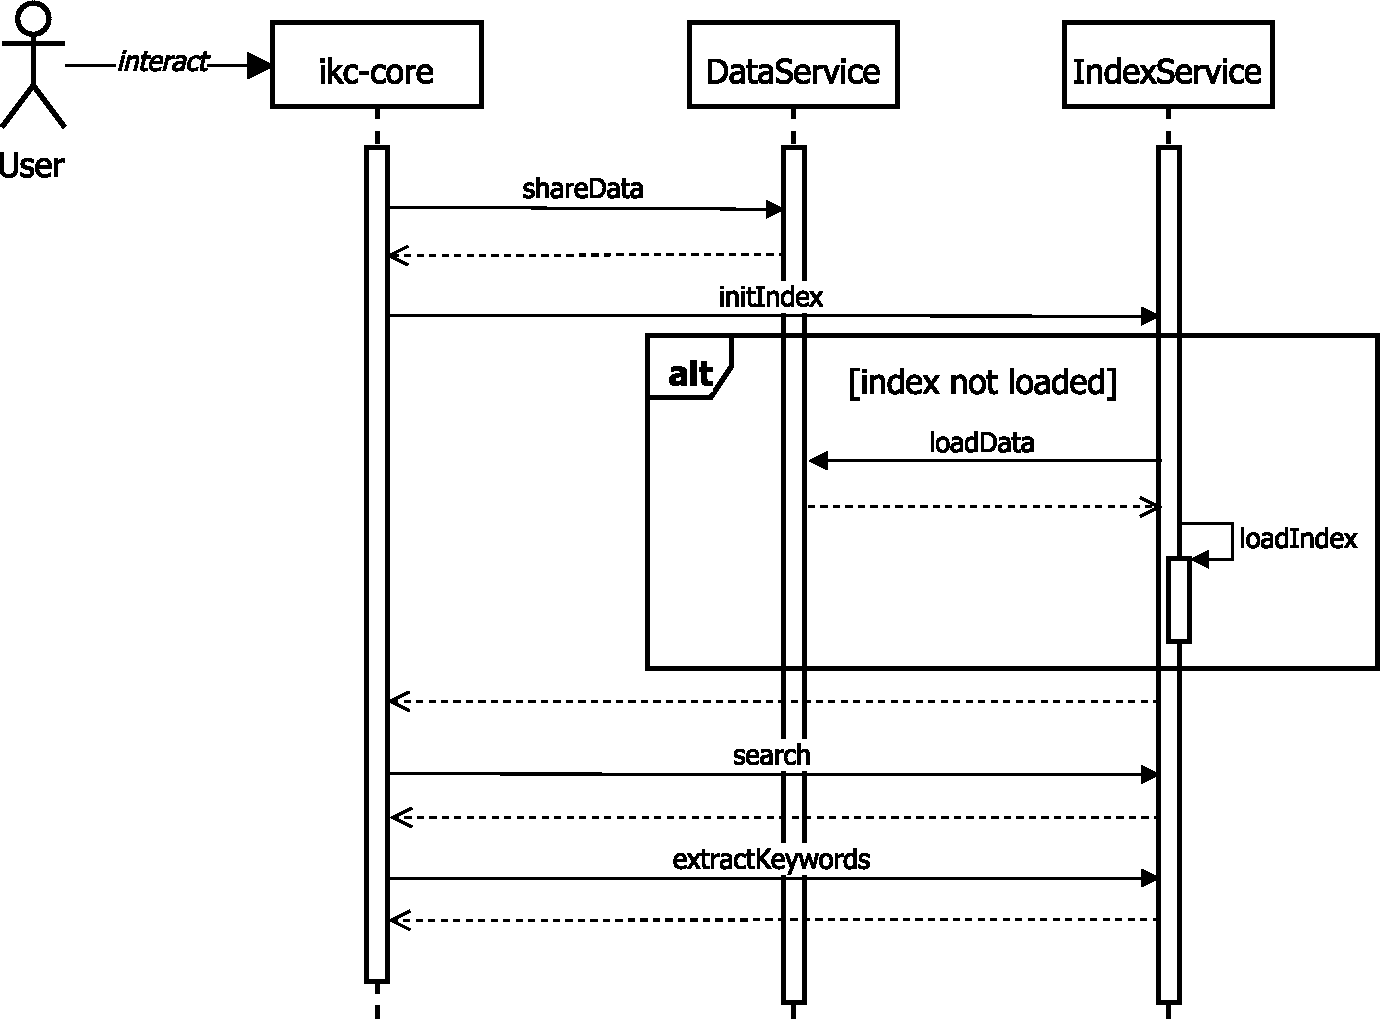
\includegraphics[width=1\textwidth]{BDA_Sequence}
\caption{Ablaufsicht}
\label{fig:ablaufsicht}
\end{figure}

Die erhaltene Freigabe gibt der \gls{ikc-core} im Prozess \texttt{initIndex} an den \texttt{IndexService} weiter. Hat dieser den angeforderten Index bereits geladen, gibt er diesen an den \gls{ikc-core} zurück. Ist dies nicht der Fall, holt er sich beim \texttt{Data\-Service} wiederum die benötigten Daten (\texttt{loadData}). Diese können denselben Inhalt wie oben haben. Das ist abhängig davon, ob er Index bereits erstellt wurde. Falls nicht, muss dieser auf Basis aller Dateien erstellt werden. Ist er bereits erstellt oder nach dessen Erstellung wird dies an den \gls{ikc-core} gemeldet.

Nun kann der \gls{ikc-core} die Funktionalität des \texttt{IndexService} nutzen: Er hat Zugriff auf die Volltextsuche (\texttt{search}) und die extrahierten Schlüsselwörter (\texttt{extractKeywords}). 

\subsection{Verteilung}

Wie oben schon angesprochen, findet die Entwicklung sowohl client- als auch serverseitig statt. \autoref{fig:verteilung} gibt einer detaillierten Üb\-er\-blick. Auf der Seite des Clients läuft der \gls{ikc-core} im Browser. Dieser verwendet für die Zwischenspeicherung von Daten eine \gls{in-browser Datenbank}

    
        \begin{figure}[H]
    \centering
    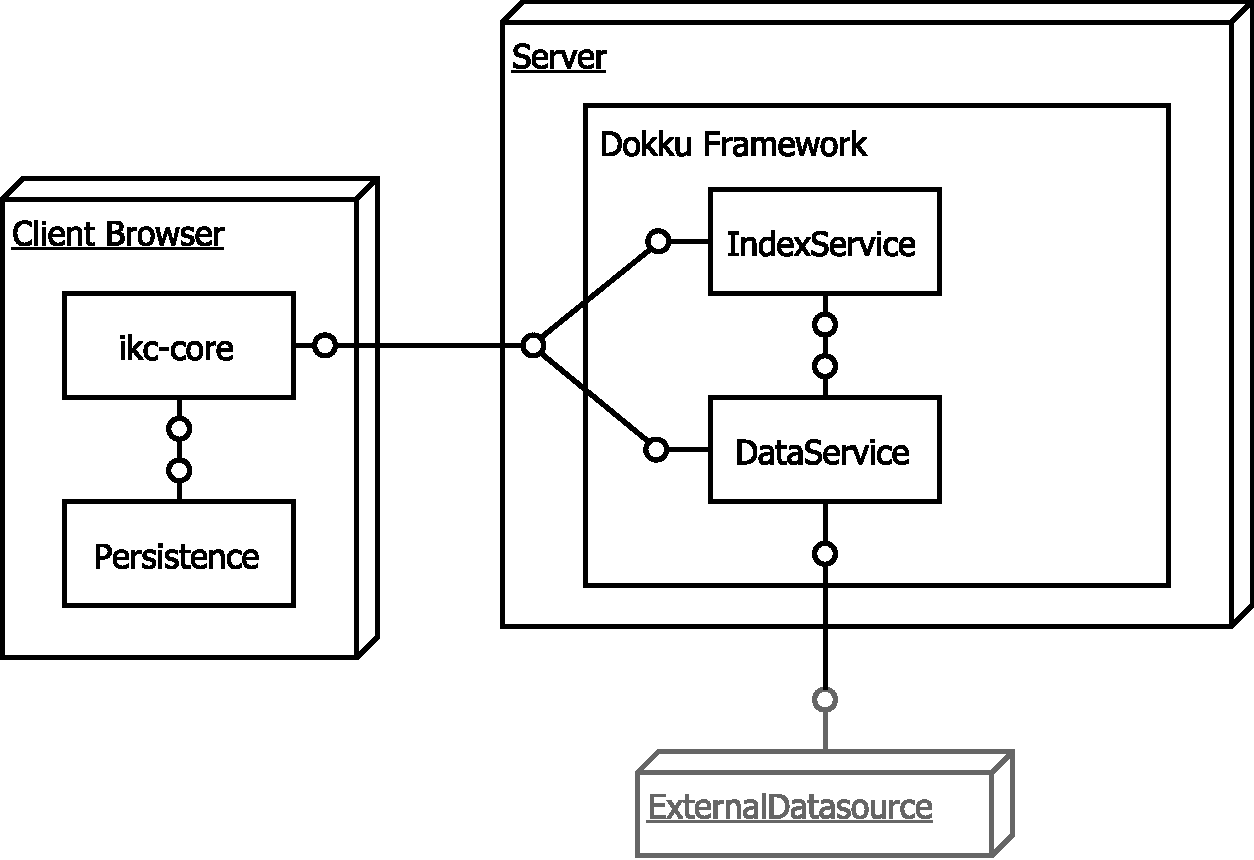
\includegraphics[width=0.7\textwidth]{DistributionView}
    \caption{Verteilung}
    \label{fig:verteilung}
    \end{figure}

% ----------------------------------------------------------------




% ----------------------------------------------------------------

\section{Algorithmus}\label{algo}

% ----------------------------------------------------------------
Der Kern des Prototyps bilden die verschiedenen Algorithmen. Basierend auf den externen Datenquellen ermöglichen sie eine Volltext-Suche und die Extraktion der relevanten \gls{Keyphrase}[s]. Nachfolgend werden die Funktionsweise als auch wichtigsten Überlegungen dazu veranschaulicht. Basierend auf verschiedenen bestehenden Ansätzen wird die Lösungsfindung für den hier verwendeten Algorithmus dargelegt. 

Um die relevanten \gls{Keyphrase}[s] für ein spezifisches Dokument zu extrahieren, werden verschiedene Methoden aus dem Feld von \hyperref[natural-language-processing]{\textit{Natural Language Processing}} kombiniert mit statistischen Analsysen und heuristischen Vorgaben. Für die Analyse der \gls{Keyphrase}[s] werden \gls{N-Gramm}[e] der Grösse eins bis vier berücksichtigt. Nebst möglichst treffenden Resultaten liegt der Fokus auch auf der raschen Aussortierung von ungeeigneten Kandidaten. Da die Berechnung der Relevanz der Rechen- und Speicher-intensivste Vorgang des Algorithmus ist, kann die Gesamtleistung des Algorithmus durch frühe Aussscheidung unnötiger Kandidaten enorm gesteigert werden. Die Anzahl möglicher \gls{N-Gramm}[e] ist definiert als: 
\[f(x)=\sum_{n=0}^N x - n  =
\begin{cases} 
   (x - n)  & \text{if } x > n \\
   0      & \text{if } x \leq n
  \end{cases}\]
Wobei $N$ die maximale Länge eines \gls{N-Gramm}[s] und $x$ die Länge des Textes repräsentieren.

In der \autoref{fig:seq_keywordextraction} werden dafür der konzeptionelle Ablauf graphisch dargestellt und anschliessend die verschiedenen Elemente genauer erläutert.

    \begin{figure}[H]
    \centering
    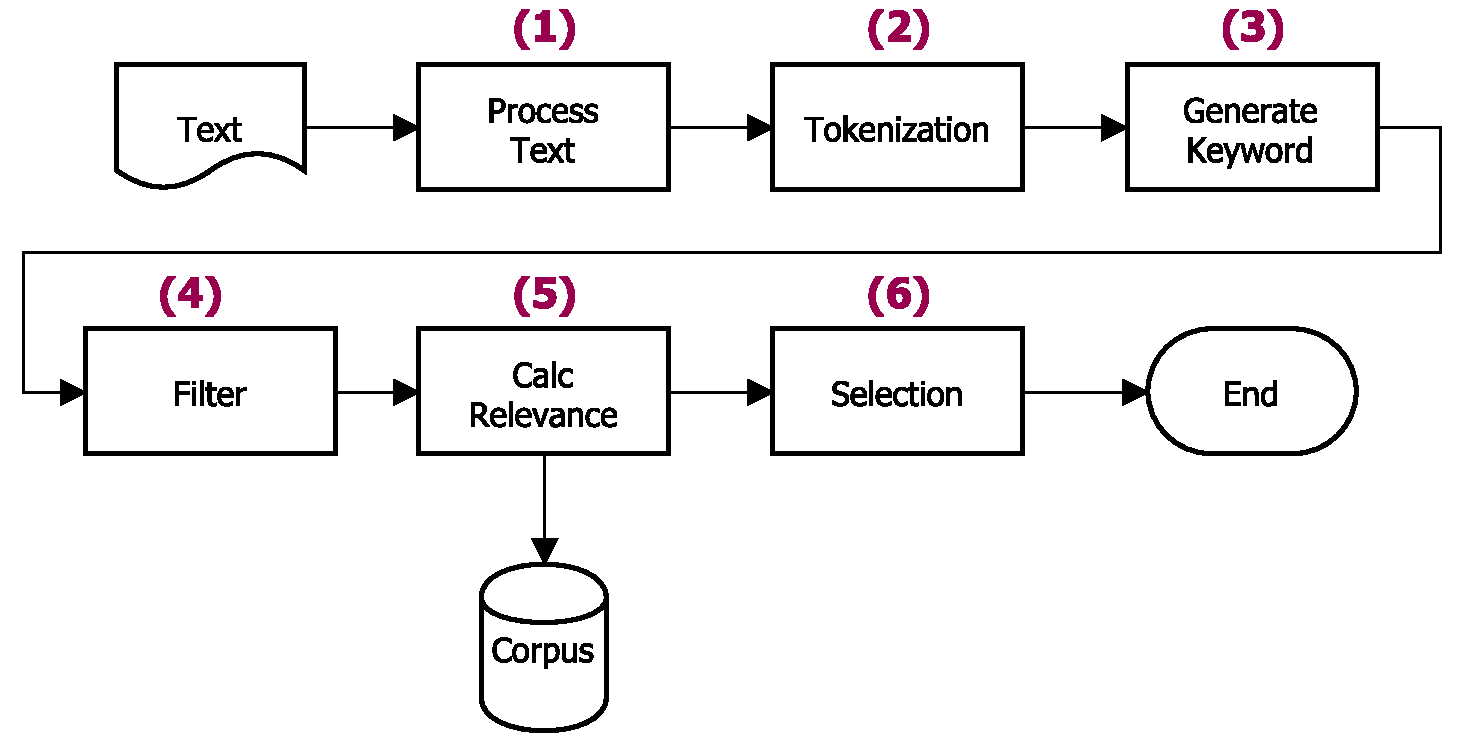
\includegraphics[width=1\textwidth]{KeywordExtraction}
    \caption{Ablauf Schlüsselwort-Extraktion}
    \label{fig:seq_keywordextraction}
    \end{figure}
 
 
 
% ----------------------------------------------------------------

\subsection{Eingabe}

% ----------------------------------------------------------------

Als Eingabe in den Algorithmus wird ein Text erwartet. Im Fall dieses Prototyps handelt es sich um einen Wikipedia-Artikel aus den Trainingsdaten. Um die folgenden Schritte besser zu illustrieren, wird der folgende Satz als Beispieltext verwendete. Mit einer Länge von $19$ Wörter, besitzt er $70$ mögliche \gls{N-Gramm}[e] mit Länge eins bis vier.

\begin{quote}
\textit{The Guardian newspaper was founded in 1821 as \glqq The Manchester Guardian\grqq, which head office is still located in Manchester.}
\end{quote}
Mit einer Länge von $19$ Wörtern besitzt er $70$ mögliche \gls{N-Gramm}[e] mit einer Länge von eins bis vier.

% ----------------------------------------------------------------

\subsection{Vorverarbeitung (1)}

% ----------------------------------------------------------------

Im ersten Schritt wird der Text anhand verschiedener Vorgaben vorbereitet. Dazu werden zu Beginn die Buchstaben nach einem Punkt, einem Fragezeichen, Ausrufezeichen oder einer Zeilenschaltung in die Kleinschreibung umgewandelt. Dies dient dazu Wörter zu erkennen, welche als Nomen genutzt werden, jedoch nicht aus dieser Wortart stammen. Dadurch verändert sich der Beispielsatz geringfügig. 

\begin{quote}
\textit{\textbf{t}he Guardian newspaper was founded in 1821 as \glqq The Manchester Guardian\grqq, which head office is still located in Manchester.}
\end{quote}

Weiter wird nun der Text in Fragmente aufgeteilt. Dabei wird davon ausgegangen, dass sich relevante \gls{Keyphrase}[s] nicht über ein Satzzeichen erstrecken. Es entsteht eine Abfolge von Textfragmenten.
\begin{quote}
\textit{\textbf{(}the Guardian newspaper was founded in 1821 as\textbf{)} \textbf{(}The Manchester Guardian\textbf{)} \textbf{(}which head office is still located in Manchester\textbf{)}}
\end{quote}
Nach dem ersten Schritt wurde der Text mit $19+18+17+16=70$ möglichen \gls{N-Gramm}[en] in eine Liste von Textfragmenten mit $(8+7+6+5)+(3+2+1)+(8+7+6+5)=58$ möglichen \gls{N-Gramm}[en] transformiert. Dadurch konnten bereits $12$ Kandidaten ausgeschlossen werden.

% ----------------------------------------------------------------

\subsection{Text Zerlegung (2)}

% ----------------------------------------------------------------

Vor der Bildung der eigentlichen Kandidaten werden nun die Textfragmente durch \hyperref[tokenization]{\textit{Tokenization}} in eine Liste von einzelnen Wörter aufgeteilt. Ebenfalls werden dabei unerwünschte Sonderzeichen am Anfang oder am Ende eines Wortes entfernt. Dabei handelt es sich in erster Linie um alle anderen Satzzeichen, welche bei der Aufteilung des Textes in Text-Fragmente nicht berücksichtigt wurden.

\begin{quote}
\textit{\textbf{[}the, Guardian, newspaper, was, founded, in, 1821, as\textbf{]}, \textbf{[}The, Manchester, Guardian\textbf{]}, \textbf{[}which, head, office, is, still, located, in, Manchester\textbf{]}}
\end{quote}


% ----------------------------------------------------------------

\subsection{Generierung möglicher Keyphrases (3)}

% ----------------------------------------------------------------

Anhand der generierten Wortlisten können nun die verschiedenen \gls{N-Gramm}[e] generiert werden. Es entsteht eine Liste von \gls{N-Gramm}[en] der Länge von eins bis vier.

\begin{quote}
\textit{\textbf{[}the Guardian newspaper was, the Guardian newspaper, the Gu\-ardian, the, ... , located in Manchester, located in, located, in Manchester, in, Manchester\textbf{]}}
\end{quote}


% ----------------------------------------------------------------

\subsection{Filter mittels POS-Tagger (4)}

% ----------------------------------------------------------------

Wie von \cite{parameswaran2010towards} beschrieben, folgen relevante \gls{Keyphrase}[s] bestimmten grammatikalischen Regeln. Diese sind wie folgt definiert:
\begin{enumerate}
    \item Eine relevante \gls{Keyphrase} besteht mindestens aus einem Nomen. Somit entfallen \gls{Keyphrase}[s] wie zum Beispiel \textit{was} oder \textit{located in}.
    \item Eine relevante \gls{Keyphrase} beginnt nicht mit einem Pronomen, einem Verb oder einem Partikel. Diese Regel sortiert \gls{Keyphrase}[s] wie \textit{the Guardian newspaper} aus.
    \item Eine relevante \gls{Keyphrase} endet nicht mit einem Pronomen, Verb oder Partikel. Diese Regel sortiert zusätztlich \gls{Keyphrase}[s] wie \textit{Guardian newspaper was} aus.
\end{enumerate}

Allerdings gibt es auch Ausnahmen: Es existieren \gls{Keyphrase}[s], welche kein eigentliches Nomen enthalten. In der englischen Sprache gibt es beispielsweise zahlreiche Eigennamen, welche ebenfalls potentielle \gls{Keyphrase}[s] darstellen können. Diese beginnen oft mit einem Grossbuchstaben. Also kann weiter folgende Regel definiert werden:

\begin{enumerate}
    \item[4.] Eine relevante \gls{Keyphrase} beginnt mit einem Grossbuchstaben. Wie bereits erwähnt, wurden vorgängig Wörter innerhalb des Textes nach bestimmten Satzzeichen in die Kleinschreibung umgewandelt. Dieser Vorgang schliesst diese Wörter von dieser Regel aus. Dadurch wird zum Beispiel \textit{The Manchester Guardian} weiter beachtet, auch wenn es grundsätzlich der zweiten Regel widerspricht, da diese mit einem Pronomen startet. 
\end{enumerate}

Um diese Regeln umszusetzen, wird ein \hyperref[part-of-speech]{Part-Of-Speech-Tagger} verwendet. Dabei handelt es sich um einen Algorithmus, welcher die Wortarten von gegebenen Wörtern bestimmt. Um den Regeln zu entsprechen, muss eine \gls{Keyphrase} sowohl Regeln eins und drei folgend, zusätzlich entweder der Regel zwei, Regel vier oder beiden folgen. Mittels dieser drei Regeln können alle möglichen Kandidaten, ausser den folgenden ignoriert werden:

\begin{quote}
\textit{\textbf{[}Guardian newspaper, Guardian, newspaper, 1821, The Manchester Guardian, The Manchester, The, Manchester Guardian, Manchester, Guardian, head office, head, office, Manchester\textbf{]}}
\end{quote}

Damit bleiben noch $14$ mögliche \gls{Keyphrase}[s] von ursprünglich $70$. Nun werden gleiche \gls{Keyphrase}[s] zusammengefasst, indem sie zusammen mit der jeweiligen Anzahl Vorkommnisse kombiniert werden. Das reduziert die Anzahl unterschiedlicher \gls{Keyphrase}[s] auf $12$ (\autoref{keyword-with-count}). Ebenfalls wird jeweils das erste Wort einer \gls{Keyphrase} kleingeschrieben, falls es sich nicht um ein Nomen handelt. So kann sichergestellt werden, dass zum Beispiel das 1-Gramm \glqq The\grqq\,im nächsten Schritt tiefer bewertet wird. Da die Grossschreibung nur im Kontext der \gls{Keyphrase} \textit{The Manchester Guardian} von Bedeutung ist.

\begin{longtable}{|p{4cm}| p{1cm}|}
  \hline
    \gls{Keyphrase} & \#\\\hline
    Guardian & 2  \\\hline
    Manchester & 2  \\\hline
    Guardian newspaper & 1  \\\hline
    newspaper & 1  \\\hline
    1821 & 1  \\\hline
    the Manchester Guardian & 1  \\\hline
    the Manchester & 1  \\\hline
    the & 1  \\\hline
    Manchester Guardian & 1  \\\hline
    head office & 1  \\\hline
    head & 1  \\\hline
    office & 1  \\\hline
        \caption{Keyphrase mit Anzahl Vorkommnissen}
    \label{keyword-with-count}
\end{longtable}


% ----------------------------------------------------------------

\subsection{Berechnung der Relevanz (5)}\label{calcrelevance}

% ----------------------------------------------------------------

Um die verschiedenen \gls{Keyphrase}[s] zu gewichten, wird ein individueller \gls{Score} pro \gls{Keyphrase} ausgerechnent. Dazu werden folgende Metriken benötigt (\autoref{metric-per-keyword}).

\begin{longtable}{|p{2cm}| p{8cm}|}
  \hline
    Metrik & Erläuterung\\\hline
    $numDocs$ & Anzahl Dokumente im Korpus. \\\hline
    $corpFreq$ & Häufigkeit des \gls{Keyphrase}[s] innerhalb des Korpus. \\\hline
    $docLength$ & Anzahl Wörter des spezifischen Dokumentes. \\\hline
    $freq$ & Häufigkeit der \gls{Keyphrase} innerhalb des Dokuments. \\\hline
    \caption{Benötigte Metriken}
    \label{metric-per-keyword}
\end{longtable}


Basierend auf den eingeführten Metriken wird mit Hilfe einer angepassten Version der \textit{Similarity}-Formel\footnotemark \footnotetext{\cite{TFIDFSim65:online}} des \textit{Apache Lucene} Projekts gearbeitet. Die verwendet Formel für die Berechnung des \gls{Score}[s] sieht folgendermassen aus:

\begin{equation}\label{tf}
tf = freq
\end{equation}
\begin{equation}\label{idf}
idf  =  1 +log( \frac{numDocs}{1 + corpFreq})
\end{equation}
\begin{equation}\label{lengthNorm}
lengthNorm =\frac{1}{docLength} 
\end{equation}
\begin{equation}\label{tfidf}
tfidf = tf * idf * lengthNorm
\end{equation}

\autoref{tf} repräsentiert die Häufigkeit der \gls{Keyphrase} innerhalb des gegebenen Dokuments. Wenn sich Anzahl erhöht, steigt auch der \textit{tf}-Wert. Um den Einfluss diese Faktors zu reduzieren, wird der Wert mittels der Wurzelfunktion etwas gedämpft.

Neben der Häufigkeit innerhalb des Dokuments ist die inverse Häu\-fig\-keit (\autoref{idf}) ein wichtiger Wert. Diese basiert auf den Vorkommnissen einer \gls{Keyphrase} über den gesamten Korpus. Dadurch wird die Einzigartigkeit der \gls{Keyphrase} innerhalb des Korpus ausgedrückt. Dieser Wert sinkt, je öfter die gleiche \gls{Keyphrase} in anderen Dokumenten enthalten ist. Mittels der Addition von eins im Nenner innerhalb der Logarithmus-Funktion wird eine Division durch Null verhindert. 

%Würde der Score mittels der \autoref{tf} und der \autoref{idf} berechnet werden, so würden kurz und lange Dokumente Werte in anderen Bereichen produzieren. Eine Verwendung eines Schwellwertes zur Begrenzung der Anzahl \gls{Keyphrase}[s] wäre unmöglich. Dazu wird der Wert mit Hilfe der Dokumentenlänge normalisiert. Dazu wird mittels der \autoref{lengthNorm} der \gls{Score} normalisiert


Würde der \gls{Score} lediglich mit den beiden Faktoren \autoref{tf} und \autoref{idf} berechnet, so wären die berechneten \gls{Score}[s] aus Dokumenten mit unterschiedlicher Textlänge nicht vergleichbar. Auch die Verwendung eines Schwellenwertes für die Begrenzung der Anzahl \gls{Keyphrase}[s] wäre verunmöglicht. Eine Normalisierung über die Dokumentenlänge ist somit notwendig. Dazu wird die \autoref{lengthNorm} eingesetzt.

% ----------------------------------------------------------------

\subsection{Auswahl (6)}

% ----------------------------------------------------------------

Schlussendlich werden die berechneten \gls{Keyphrase}[s] mit Hilfe eines Schw\-el\-werts und anhand deren Inhalt begrenzt. Damit können eine sinnvolle Anzahl an Dokumenten zurückgegeben. Im Gegensatz zu einer Begrenzung der Anzahl \gls{Keyphrase}[s] kann mit einem Schwellwert je nach Text eine Anzahl an \gls{Keyphrase}[s] zurückgegeben werden, welche für den Text ideal ist. Beispielsweise macht es wenig Sinn, dass aus einem kurzen Text gleich viele \gls{Keyphrase}[s] extrahiert werden wie aus einem langem. Denn aufgrund der unterschiedlichen Länge enthalten die beiden Texte prinzipiell eher nicht gleich viel relevanten Inhalt. Weiter werden \gls{Keyphrase}[s] gefiltert welche in anderen \gls{Keyphrase}[s] enthalten sind. So werden zum Beispiel \textbf{head} und \textbf{office} gefiltert da beide im \gls{Keyphrase} \textbf{head office} enthalten sind.


% ----------------------------------------------------------------

\subsection{Dokumente für Schlüsselwort}

% ----------------------------------------------------------------

Die gegenteilige Operation der \gls{Keyphrase}-Extraktion ist die Extraktion aller Dokumente für eine bestimmte \gls{Keyphrase}. Dabei wird eine Liste an Dokumenten erwartet, in welchen eine bestimmte \gls{Keyphrase} einen hohen \gls{Score} ausweist. 

    \begin{figure}[H]
    \centering
    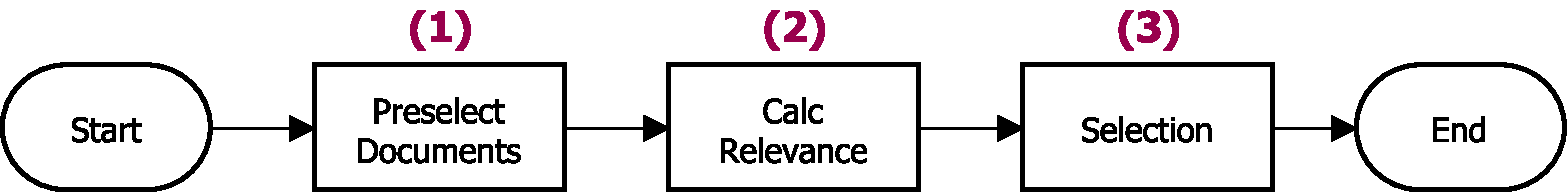
\includegraphics[width=1\textwidth]{DocumentForKeyword}
    \caption{Ablauf: relevante Dokumente für eine \gls{Keyphrase}}
    \label{fig:seqdocforkeyword}
    \end{figure}
\begin{enumerate}
    \item Dazu werden in einem ersten Schritt alle möglichen Dokumente ausgewählt. In dieser Menge an Dokumenten kommt die entsprechende \gls{Keyphrase} mindestens einmal vor, jedoch ungeachtet der Relevanz der \gls{Keyphrase}[s] für das jeweilige Dokument.
    \item In einem nächsten Schritt wird für jedes Dokument der jeweiligen \gls{Score} für die entsprechende \gls{Keyphrase} berechnet. Die Berechnung folgt dabei exakt dem bereits vorgestellten Ablauf (\autoref{calcrelevance}).

    \item Nun wird ebenfalls die Anzahl an Resultaten mit Hilfe eines Schwellwerts reduziert. Somit kann die Auswahl auf die wirklich relevanten Dokumente für die entsprechende \gls{Keyphrase} vermindert werden.
            
\end{enumerate}

% ----------------------------------------------------------------

\section{Integration des Prototypen}\label{Integration}

% ----------------------------------------------------------------

Basierend auf der ausgeführten Architektur (\autoref{architecture}) werden im folgenden Abschnitt die wichtigsten Software-Konzepte erläutert. Diese werden kurz zusammengefasst, anschliessend folgt eine Beschreibung der Integration des Prototyps in den bestehenden \gls{ikc-core}.

% ----------------------------------------------------------------

\subsection{Übersicht}

% ----------------------------------------------------------------


Im Klassendiagramm auf \autoref{fig:prototypeClassDiagram-easy} sieht man einen Überblick über den zu entwickelnden Prototypen. Abgebildet sind die wichtigsten Klassen und deren Beziehungen untereinander. Zunächst liegen die zwei Teile \gls{ikc-core} und \texttt{Prototype} vor. Der \gls{ikc-core} ist der aus dem Forschungsprojekt \gls{IKC} herausgehende bestehende Prototyp. Dieser nimmt Gebrauch von den beiden vom \texttt{Prototypen} zur Verfügung gestellten Schnittstellen des \texttt{Index-} und des \texttt{DataServices}.

Grundsätzlich besteht der \texttt{Prototyp} aus den Komponenten \texttt{Index-} und \texttt{DataService}. Diese verwenden das von ausserhalb ver\-füg\-bar\-e \texttt{MessageModel}. Es enthält die Protokolle für die jeweilige Kommunikation und wird somit auch vom \gls{ikc-core} in Anspruch genommen.

Die genauen Abläufe und auch die Implementation des \texttt{Index-} beziehungsweise \texttt{DataServices} ist unter dem Abschnitt der technischen Umsetzung (\autoref{implementation}) zu finden.

    \begin{figure}[H]
    \centering
    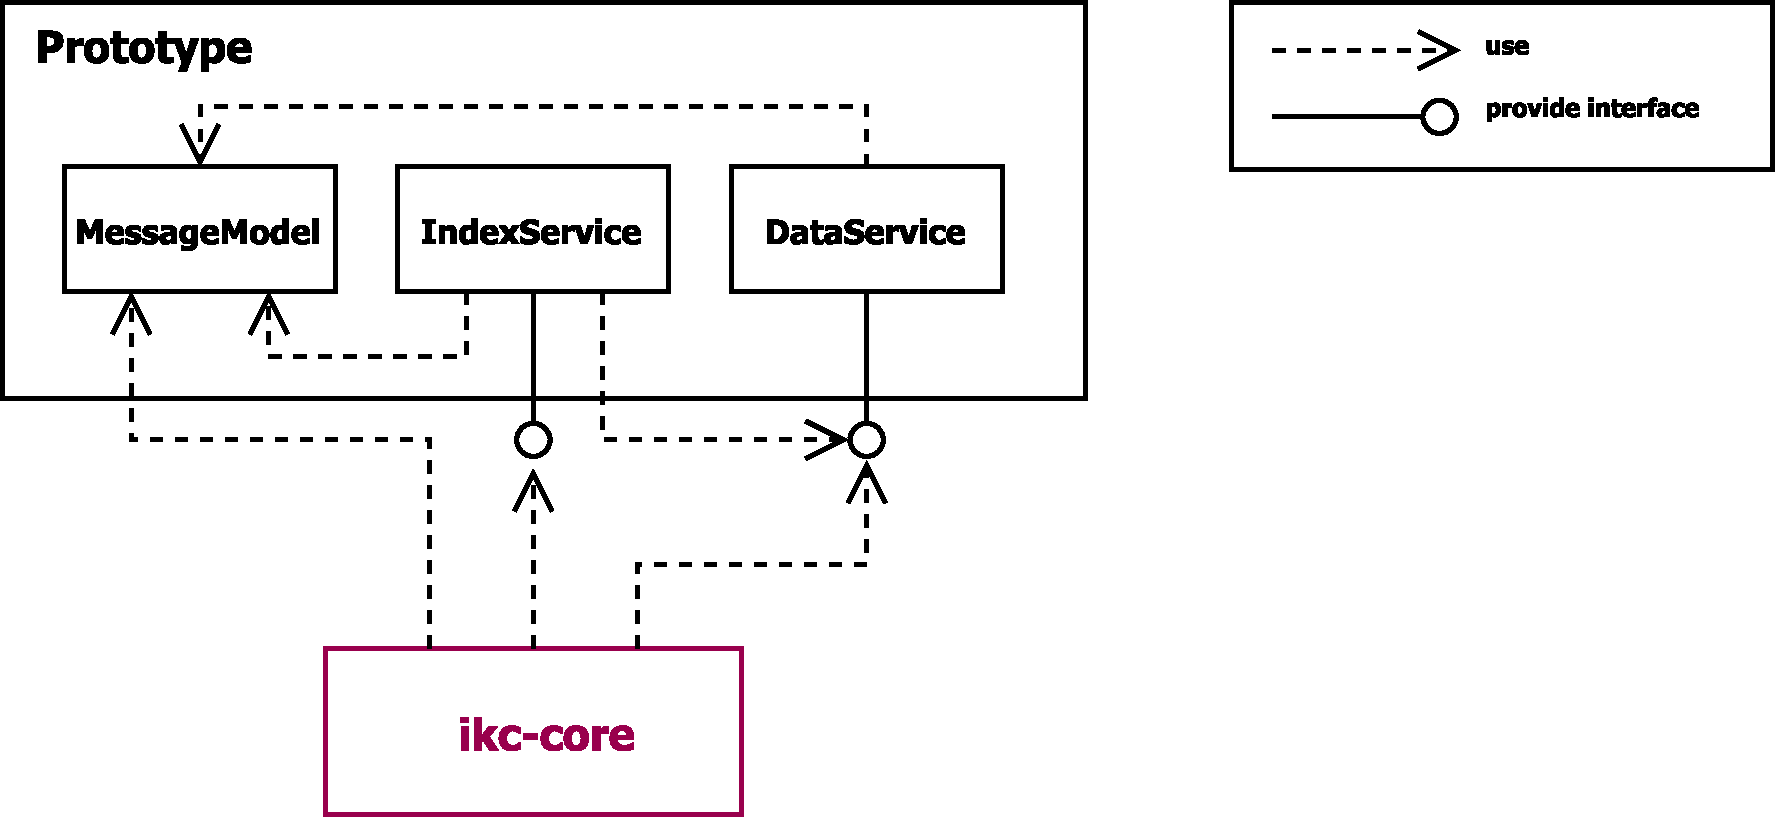
\includegraphics[width=1\textwidth]{ClassDiagrammGeneral}
    \caption{Klassendiagramm: Prototype}
    \label{fig:prototypeClassDiagram-easy}
    \end{figure}

Der Kern der Software bildet der Algorithmus. Dieser ist, neben der Suchfunktionalität und dem Aufbau der Indizes, ein Hauptbestandteil des \texttt{IndexService}. \autoref{fig:kommunikation} gewährt einen Überblick über die beteiligten Komponenten. Als Grundlage benötigt der \texttt{In\-dex\-Ser\-vice} alle zu indexierenden Dateien im Volltext. Deren Quelle ist der \texttt{Data\-Ser\-vice}. Der \texttt{Index-} und der \texttt{DataService} bilden zusammen den eigentlichen Prototypen. Wie in der Bausteinsicht auf \autoref{fig:bausteinsicht} zu erkennen, gibt es neben der Integration der Services auch eine Einbindung in die bestehende Benutzeroberfläche des \gls{ikc-core}.

% ----------------------------------------------------------------

\subsection{Schnittstellen}

% ----------------------------------------------------------------

Der Prototyp soll sich möglichst nahtlos in den \gls{ikc-core} integrieren. Um dies zu erreichen sollen in keiner Situation Funktionen des \gls{ikc-core}[s] blockiert werden durch den Prototyp. 

So werden Suchresultate des Index innerhalb der bestehenden Suche integriert und bei Bedarf aktualisiert. Die verschiedenen Resultate der unterschiedlichen Quellen sollen in Echtzeit nach ihrem Eintreffen dargestellt werden. Somit wird sich die Liste mit Resultaten trotz gleichem Suchbegriff über die Zeit verändern, da weitere Resultate von entfernten Quellen eintreffen. Bei der Auswahl eines Resultats wird es herkömmlicher Node dargestellt. 

Weiter werden extrahierte \gls{Keyphrase}[s] klar getrennt von den bestehenden Eigenschaften des Nodes als \textit{Chips} oberhalb des Titels dargestellt werden. Sowohl ein Dokument mit entsprechenden \gls{Keyphrase}[s] als auch eine \gls{Keyphrase} mit den verknüpften Dokumenten werden als Node dargestellt. \autoref{fig:bda-integration} zeigt einen Entwurf dieser Integration. 

    \begin{figure}[H]
    \centering
    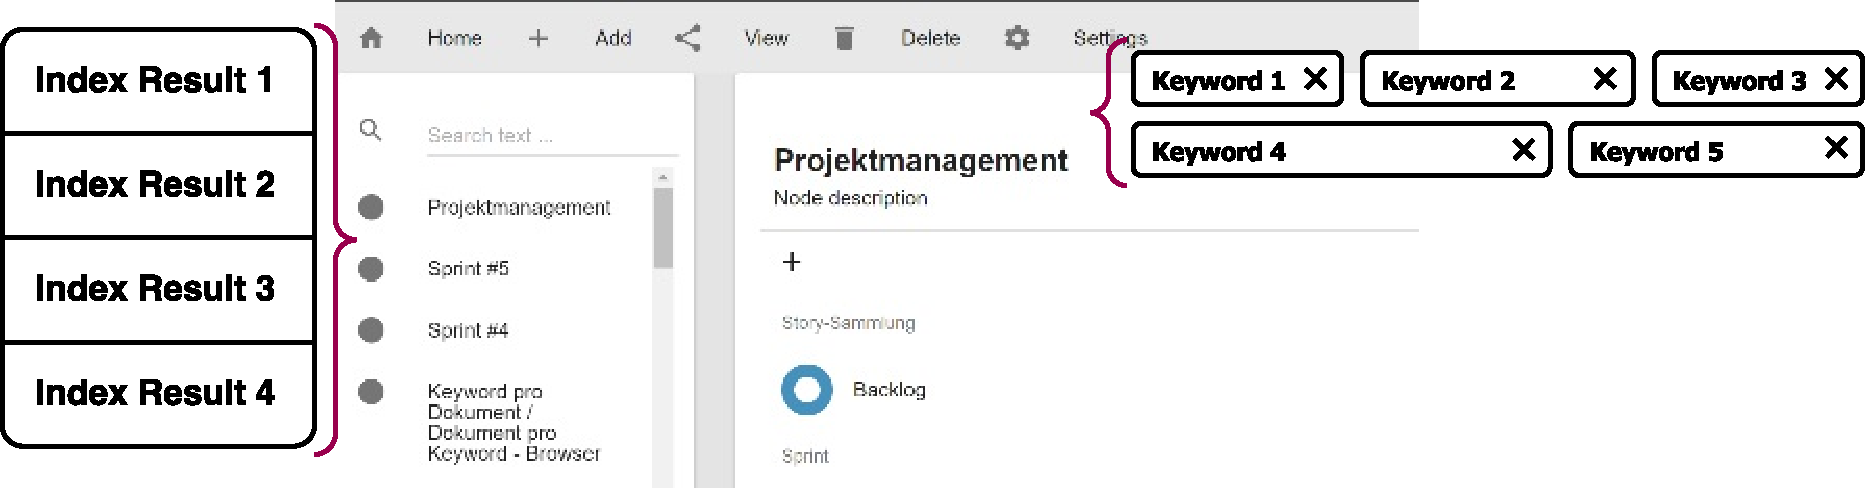
\includegraphics[width=1\textwidth]{BDA_UI}
    \caption{Entwurf Integration Benutzeroberfläche}
    \label{fig:bda-integration}
    \end{figure}

Um die Schnittstellen des Prototyps ideal zu verwenden und die obigen Oberflächenanpassungen umzusetzen, sind Anpassungen beziehungsweise Erweiterungen in der Software-Struktur des \gls{ikc-core} nötig. 

Auf obigem Klassendiagramm (\autoref{fig:prototypeClassDiagram-easy}) ist ersichtlich, dass sowohl der \texttt{IndexService}, als auch der \texttt{DataService} externe Schnittstellen bereithalten.



%riesiges index.json, ungefähr 100k Files als Text-Dateien

% ----------------------------------------------------------------

\section{Datenfreigabe}\label{l-datenfreigabe}

% ----------------------------------------------------------------


Für den Auftraggeber ist eine sichere Kommunikation, stetige Transparenz und Kontrolle über den Verbleib von benutzergenerierten Daten von hoher Wichtigkeit. Um diesen Anforderungen gerecht zu werden, wurde unter anderem ein Datenfreigabe-Konzept entwickelt. Dieses basiert auf Einweg-\gls{Token}[s], welche als Schlüssel für die Freigabe verwendet werden.  Dabei fordert einen \textit{Accessor} beim \textit{Provider} den Zugriff auf eine Ressource an. Der \textit{Provider} hält dabei die Informationen für den Zugriff auf die Ressourcen und der \texttt{DataService} regelt den tasächlichen Zugriff auf die Ressource. In \autoref{fig:seqaccesssession-easy} ist der Ablauf genauer aufgezeigt:
\begin{itemize}
    \item Als erster Schritt fordert der \textit{Accessor} beim \textit{Provider} Zugriff auf eine Ressource.
    \item Der \textit{Provider} sendet nun die nötigen Informationen für die Verbindung auf die Ressource an den \textit{DataService} und fordert einen Token.
    \item Sobald der Token generiert wurde, erhält der \textit{Provider} dieser und sendet ihn an den \textit{Accessor}.
    \item Anschliessend kann der \textit{Accessor} mithilfe des Token beim \texttt{Da\-ta\-Ser\-vi\-ce} den Inhalt der Ressource anfragen.
    \item Beim Erhalt eines Token überprüft nun den \texttt{DataService} den Token auf deren Gültigkeit überprüft. Ist der Token gültig, werden die Daten anhand der Informationen zur Verbindungen von der externen Datenquelle bezogen und an den \textit{Accessor} geliefert. Anschliessend wird der Token gelöscht, so dass er nicht wiederholt verwendet werden kann.
\end{itemize}

%ablaufdiagramm Einwegtoken Entkopplung

    \begin{figure}[H]
    \centering
    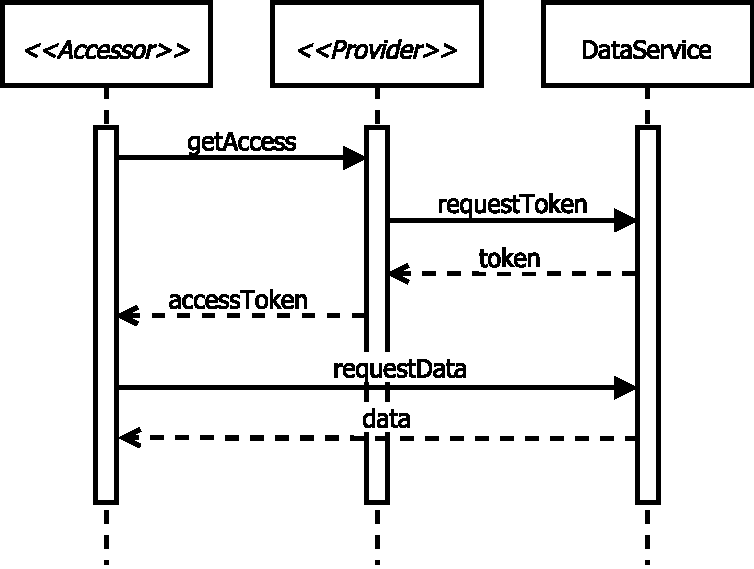
\includegraphics[width=0.8\textwidth]{SeqAccessGeneral}
    \caption{Ablauf: Datenfreigabe}
    \label{fig:seqaccesssession-easy}
    \end{figure}

% ----------------------------------------------------------------

\section{Auto-Indexierung}

% ----------------------------------------------------------------

Durch die Auto-Indexierung der externen Datenquellen, wird die Volltext-Suche möglich und bietet die Grundlage für die \gls{Keyphrase}-Extraktion. Die Indexierung der Datenquellen, wird durchgeführt sobald der Benutzer die entsprechenden Berechtigungen hinterlegt hat. Dazu werden sämtliche Elemente geladen und verarbeitet. Falls schon ein Index existiert, wird dieser eingelesen und mit den ge\-än\-der\-ten oder neuen Elemente aktualisiert. Der Index ist aufgeteilt in zwei Bereiche: Zum einen der Suche-Index, welcher mit Hilfe der Bibliothek \gls{elasticlunr} erstellt wird. Zum anderen hält der Frequenz-Index die möglichen \gls{Keyphrase}[s] zusammen mit Ihrer Frequenz im Korpus und den jeweilig Dokumente, welche das \gls{Keyphrase} enthalten.

% ----------------------------------------------------------------

\section{Variantendiskussion}

% ----------------------------------------------------------------


Basierend auf dem Stand der Technik (\autoref{literatur}) wurden verschiedene Optionen für die Umsetzung nötiger Funktionen getestet und evaluiert. Dieser Abschnitt zeigt die grundlegenden Gründe und Üb\-er\-le\-gun\-gen, welche für oder gegen eine Bibliothek oder allgemein eine Variante sprechen.


% ----------------------------------------------------------------

\subsection{Algorithmus}

% ----------------------------------------------------------------

Die Berechnung der Relevanz (\autoref{calcrelevance}) ist eine der zentralsten Aufgaben des Algorithmus. Die Schwierigkeit dabei liegt in der benötigten Ausgewogenheit der gesuchten Formel. Die relevante \gls{Keyphrase}[s] sollen sowohl spezifisch für den jeweiligen Text sein, jedoch auch ein gewisse Generalisierung aufweisen. Dazu wurden verschiedenen Varianten geprüft:

\begin{itemize}
    \item Die Standard \textit{TF-IDF} (\autoref{default}) ist eine der verbreitetsten Formeln zur Berechnung der Relevanz. Sie ist leicht zu berechnen und gut geeignet für eine Suche oder die Bestimmung von ähnlichen Dokumenten. Jedoch ist sie nicht normalisiert und somit ist der Vergleich von Dokumenten unterschiedlicher Längen eher schwer. Dies wird aber benötigt, um einen einheitlichen Schwellenwert für relevante \gls{Keyphrase}[s] zu definieren. Weiter können sehr spezifische Begriffe extrem hoch gewertete \gls{Keyphrase}[s] werden. Obwohl sie für eine Abstraktion des Textes nicht optimal sind. 
    \begin{equation}\label{default}
    \underbrace{termDocFreq}_\text{\textbf{TF}} * \underbrace{ (1 +log( \frac{numDocs}{1 + docFreq}))}_\text{\textbf{IDF}}
    \end{equation}
    \item Basierend auf der \autoref{default} wird bei der \autoref{default-modified} der \textit{IDF} Wert mit der Häufigkeit (\textit{termFreq}) des \gls{Keyphrase} innerhalb des Korpus berechnet und nicht mit der Anzahl Dokumente (\textit{docFreq}), welche diese \gls{Keyphrase} enthält. 
    \begin{equation}\label{default-modified}
    \underbrace{termDocFreq}_\text{\textbf{TF}} *  \underbrace{ (1 +log( \frac{numDocs}{1 + termFreq}))}_\text{\textbf{IDF}} 
    \end{equation}
    \item Die \autoref{default-modified-norm} erweitert die \autoref{default-modified} mit einer Normalisierung. Dadurch werden \gls{Keyphrase}[s] von Dokumenten verschiedener Längen vergleichbar. Dabei wird der \textit{TF} Wert durch die Länge des jeweiligen Dokument dividiert.
    \begin{equation}\label{default-modified-norm}
    \underbrace{ \frac{1}{length} }_\text{\textbf{norm}}  * \underbrace{termDocFreq}_\text{\textbf{TF}} *  \underbrace{ (1 +log( \frac{numDocs}{1 + termFreq}))}_\text{\textbf{IDF}}
    \end{equation}
    \item \autoref{lucene} beschreibt eine von \gls{Lucene} verwendete Formel zur Berechnung der Relevanz. Dazu wurde \textit{TF-IDF} als Grundlage verwendet und angepasst. Hierfür wurde anstelle des \textit{TF}-Wertes, die Wurzel davon und als Ersatz des \textit{IDF}-Wertes das Quadrat des \textit{IDF}-Wertes verwendet. Weiter wurde eine Normalisierung eingeführt, dazu wird der gesamte Term durch die Wurzel der Textlänge dividiert. Mit diesen Anpassungen wurde der Stellenwert des \textit{IDF}-Wertes erhöht, damit werden automatisch \gls{Keyphrase}[s], welche sehr selten in anderen Dokumenten vorkommen höher gewichtet. Dies geschieht durch die Quadrierung des \textit{IDF}-Wertes und der Radizierung des \textit{TF}-Wertes.
    \begin{equation}\label{lucene}
    \underbrace{ \frac{1}{sqrt(length)} }_\text{\textbf{norm}} * sqrt(\underbrace{termDocFreq}_\text{\textbf{TF}}) *  (\underbrace{(1 +log( \frac{numDocs}{1 + termFreq}))}_\text{\textbf{IDF}})^{2}
    \end{equation}
\end{itemize}

% ----------------------------------------------------------------

\subsection{Kommunikation}

% ----------------------------------------------------------------

Wiederum beschäftigt sich der Abschnitt Kommunikation mit der grundlegenden Infrastruktur zum Austausch von Informationen. \autoref{l-datentransfer} geht anschliessend auf die Form ein, in welcher die Daten effektiv ausgetauscht werden.


% ----------------------------------------------------------------

\subsubsection{Websocket}

% ----------------------------------------------------------------

Für den Transport über das Netzwerk sind \gls{Websocket}[s] eine erste Möglichkeit. Im Umgang mit kleinen Dateien sind \gls{Websocket}[s] eine einfache und schlanke Lösung. Für grosse Dateien sind sie alleine aber nicht ausreichend, da man schnell den verfügbaren Arbeitsspeicher überschreitet und auch die maximale String-Länge begrenzt ist. Für den Umgang mit grossen Dateien ist somit die Verwendung von \gls{Stream}[s] und \gls{Buffer}[s] Pflicht. 


% ----------------------------------------------------------------

\subsubsection{Stream}

% ----------------------------------------------------------------

Für einen asynchronen Datentransfer von grösseren Dateien über das Netzwerk sind \gls{Stream}[s] nötig. Sie funktionieren prinzipiell analog zu grundlegenden \gls{Stream}[s] in Unix-Systemen. \gls{Stream}[s] teilen die Gesamtheit der zu sendenden oder zu empfangenden Daten in eine Sequenz von kleineren Daten auf. Die Übertragung verläuft kontinuierlich.

Die Verwendung von \gls{Stream}[s] auf Basis von \gls{Websocket}[s] führ\-te mit der Bi\-blio\-thek \textit{websocket-stream}\footnote{\url{https://github.com/maxogden/websocket-stream}} leider ebenfalls nicht zum Erfolg. Die Verwendung der verschiedenen \gls{Stream}[s] Probleme führte zu Problemen, wessen Ursprung nicht gefunden werden konnte.

Zu diesem Zeitpunkt war festgelegt, dass für die Übermittlung definitiv Streams verwendet werden müssen. Also konnte die Recherche zumindest weiter eingeschränkt werden. Der Fokus wurde auf Bibliotheken gesetzt, welche auf Websockets und Streams basieren.


% ----------------------------------------------------------------

\subsubsection{Bibliotheken}

% ----------------------------------------------------------------


Websockets als Grundlage erscheinen sinnvoll. Allerdings kann deren Verwendung mit Hilfe von Zusatzbibliotheken vereinfacht und deren Funktionalität erweitert werden.

\textit{Delivery.js}\footnote{\url{https://github.com/liamks/Delivery.js}} war die nächste interessante Bibliothek. Der Status \glqq Experimental\grqq war nicht der Grund für den Entscheid gegen diese Bibliothek. Vielmehr ist sie für eine Verwendung direkt mit \texttt{FileStreams}, also direkt mit der \texttt{I/O} vorgesehen. Zwar werden im Prototypen auch \texttt{FileStream} verwendet, jedoch werden die \gls{Stream}[s] nicht direkt über das Netzwerk weitergeleitet, sondern die einzulesenden Daten müs\-sen zusätzlich noch verändert werden. \textit{Delivery.js} grundsätzlich basiert auf \texttt{no\-de-stre\-ams} und \texttt{socket.io}.

Die grosse Verbreitung von \texttt{socket.io} war der Grund für eine vertiefte Recherche in diese Richtung. Schnell wurden auch diverse Zusatzbibliotheken gefunden, welche vielversprechend aussahen. \texttt{so\-cket.\-io-\-stre\-am} ist eine Erweiterung für die Verwendung von \gls{Stream}[s], welche einfach in Kombination mit \texttt{socket.io} verwendet werden kann. Sie wird als Hülle um den grundlegenden Stream gelegt. Diese Variante führte schnell zu guten Ergebnissen, wurde deshalb auch weiter eingesetzt.


% https://github.com/nkzawa/socket.io-stream
% http://msgpack.org
% https://nodejs.org/api/stream.html
% https://github.com/substack/stream-handbook
% https://books.google.ch/books?hl=de&lr=&id=YgdbZbkTDkoC&oi=fnd&pg=PT9&dq=socket.io&ots=TVDh5nhPCQ&sig=kcHauykErOKQuNAtqxfNs5JahxM#v=onepage&q=socket.io&f=false

%streams, pakete, Protokoll

% https://allesagil.net/category/projektmanagement/


% ----------------------------------------------------------------

\subsection{Datentransfer}\label{l-datentransfer}

% ----------------------------------------------------------------


Ein erster Versuch war das simple Senden von Daten über die zur Verfügung stehende Infrastruktur. Dies funktioniert bei kleinen Daten ohne interne Struktur recht einfach. Allerdings sind die Daten im vorliegenden Fall teilweise sehr gross und auch ist für eine effiziente Verarbeitung auch eine gewisse interne Struktur in Form von Message-Objekten notwendig. Diese Strukturen sollen sowohl client- als auch serverseitig verfügbar sein. Also müssen diese in irgendeiner Form mit übermittelt werden. Dazu müssen die Strukturen in eine Form gebracht werden, welche über das Netzwerk übermittelt werden kann. Dieser Prozess wird Serialisierung genannt, welcher weiter auch für die Persistenz eingesetzt werden kann. 

% ----------------------------------------------------------------

\subsubsection{JSON}

% ----------------------------------------------------------------

JSON ist ein textbasiertes Format, welche die Struktur und den Inhalt von Objekten abbildet. Es ist sehr verbreitet und in Javascript standardmässig verfügbar. Allerdings ist es für den vorliegenden Anwendungsfall nicht ideal, da es ohne weiteres nicht mit grossen Dateien umgehen kann und auch nicht sonderlich performant ist.

Ein oft gesehenes weiteres Problem ist die Verwendung von \texttt{JSON\-.parse} und oder \texttt{JSON.stringify}. Diese sind nämlich beschränkt auf die maximale String-Länge. Für die Verwendung dieser Methoden müssten die Daten somit vorgängig aufteilt werden. Andernfalls kommen diese Funktionen schnell an ihre Grenzen. Für diesen Zweck gibt es aber auch Erweiterungen:

Die Bibliothek \textit{bfj}\footnote{\url{https://github.com/philbooth/bfj}} kündigt zwar an mit grossen Dateien arbeiten zu können, verwendet im Hintergrund aber die oben genannten Funktionen, welche nicht performant im Umgang mit grossen Dateien sind und zu\-sätz\-lich ebenfallls auf die maximale String-Länge beschränkt sind.

% ----------------------------------------------------------------

\subsubsection{MessagePack}

% ----------------------------------------------------------------

Wie auch in \cite{msgpack-conf}[S.69-70] angemerkt erzielt man mit MessagePack für die Serialisierung ähnliche Resultate. Diese sind aber kleiner als mit JSON. Darum wurde hier auch MessagePack bevorzugt. MessagePack ist ebenfalls sehr verbreitet und es gibt zahlreiche Implementationen in verschiedenen Programmiersprachen.

% ----------------------------------------------------------------

\subsection{Persistenz}

% ----------------------------------------------------------------

Betreffend der Persistenz gibt es, wie im (\autoref{s-persistenz}) besprochen, unter vielen anderen Möglichkeiten Dropbox, stor.j und SFTP. Diese besitzen alle ihre spezifischen Vor- und auch Nachteile. Trotz der bereits bestehenden Basis der Anbindung an Dropbox, wurde bewusst auf die Verwendung verzichtet. Während der Entwicklung dieser Anbindung kamen immer wieder Probleme mit der Begrenzung der Zugriffe auf. Diese konnten zwar mit einer Art Stapelverarbeitung eingedämmt werden, allerdings ist die Anbindung trotzdem nicht ideal für die erwarteten grossen Datenmengen. Das Riskio von weiteren Begrenzungen und mangelnder Performance soll verhindert werden. Darum wurden Alternativen geprüft. 

Da der Projektparnter grossen Wert auf die Sicherheit und Transparenz der benutzereigenen Daten legt, ist stor.j eine interessante Option. Es basiert auf einem komplett anderen Ansatz als Dropbox oder SFTP, welcher zusätzliche Sicherheit verspricht. Bei der Entwicklung einer kleinen Demo-Anbindung konnten aber nicht alle Anforderungen erfüllt werden. Die Entwicklung der Bibliothek ist noch im Anfangsstadium. Darum wurde gegen die Verwendung entschieden. Stor.j gilt es aber sicherlich im Auge zu behalten, da die bestehenden Ansätze durchaus vielversprechend scheinen.

Schlussendlich wurde in Absprache mit dem Projektparter entschieden, dass eine SFTP-Anbindung die beste Lösung für die Entwicklung des Prototypen ist. So sind praktisch keinerlei Beschränkungen oder Risiken zu befürchten. Mit einem eigenem Server und der eigenen Anbindung sind die Möglichkeiten nahezu unbeschränkt. Der ausschlaggebende Punkte war aber der Fokus dieser Arbeit. Dieser soll nämlich auf der Volltextsuche und der Extraktion und nicht auf der Anbindung von externen Services liegen.



% begrenzt von API, grosse Datenmenge, viele Files
